\scanpage{67}
Un pantalon \inserted{(topologique)} subdivisé de façon standard, avec un ens $J$ de trous $(\operatorname{card}J=3)$ correspond à un ``triangle pondéré'' i.e.
\[
J\xrightarrow{\pi}\mathbb N
\qquad(\mathrm{NB}\ \pi(\unsure{i|j})=\text{nb d'arêtes qui relient $j$ et $k$, $i\ne j\ne k$})
\]

Carte \inserted{orientée} décomposée pantaloniquement de façon standard $\longleftrightarrow$ \deleted{\unsure{graphe}} squelette pantalonique généralisé

\deleted{i.e. carte \unsure{cellulaire} (\unsure{pas néc. orientée}) dont les sommets marqués sont d'ordre $3$ (\unsure{avec des sommets topologiques} non marqués d'ordre $1$ éventuellement), et avec une pondération des \deleted{\unsure{arêtes orientées}} \inserted{drapeaux} (\unsure{sommet} \inserted{marqué} et arête incidente) de telle façon que l'on ait pour chaque arête (cf ci-contre)}

\figure{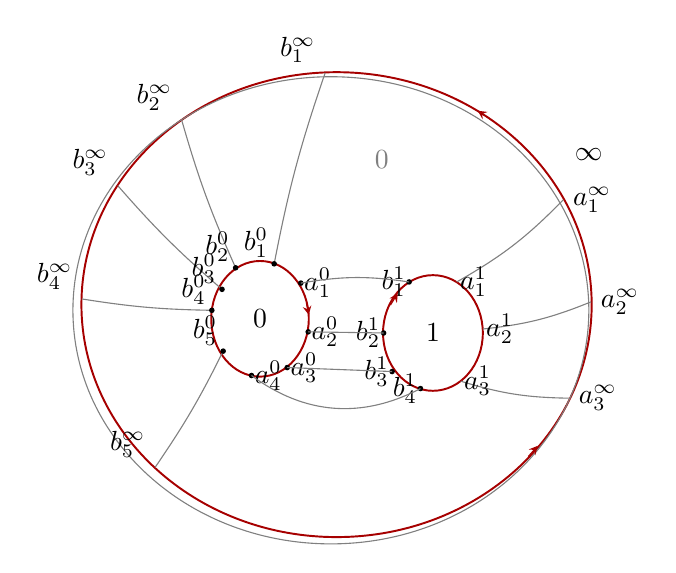
\begin{tikzpicture}[scale=.72,>=stealth]
\draw[red!65!black,line width=.7pt] (0,0) ellipse (4.5 and 4.1);
\draw[gray] (-.1,-.1) ellipse (4.55 and 4.12);
\draw[red!65!black,line width=.7pt] (-1.35,-.25) ellipse (.86 and 1.02);
\draw[red!65!black,line width=.7pt] (1.7,-.5) ellipse (.88 and 1.02);
\node at (-1.35,-.25) {$0$}; \node at (1.7,-.5) {$1$};
\node at (4.45,2.65) {$\infty$}; \node[gray] at (.8,2.55) {$\unsure{0}$};
\coordinate (B01) at (-1.1,.72); \coordinate (B02) at (-1.78,.65);
\coordinate (B03) at (-2.02,.27); \coordinate (B04) at (-2.2,-.1);
\coordinate (B05) at (-2,-.82);
\coordinate (BO1) at (-.2,4.09); \coordinate (BO2) at (-2.73,3.25);
\coordinate (BO3) at (-3.86,2.1); \coordinate (BO4) at (-4.49,.1);
\coordinate (BO5) at (-3.2,-2.87);
\foreach \i in {1,2,3,4,5}{
 \draw[gray] (B0\i) to[bend left=4] (BO\i);
 \fill (B0\i) circle (1.4pt);
 \node[above left,inner sep=2pt] at (B0\i) {$b_{\i}^{0}$};
 \node[above left] at (BO\i) {$b_{\i}^{\infty}$};
}
\coordinate (A01) at (-.63,.38); \coordinate (A02) at (-.5,-.48);
\coordinate (A03) at (-.87,-1.11); \coordinate (A04) at (-1.5,-1.25);
\coordinate (B11) at (1.28,.4); \coordinate (B12) at (.83,-.5);
\coordinate (B13) at (.98,-1.18); \coordinate (B14) at (1.48,-1.48);
\foreach \i in {1,2,3,4}{
 \fill (A0\i) circle (1.4pt); \fill (B1\i) circle (1.4pt);
 \node[right,inner sep=1pt] at (A0\i) {$a_\i^0$};
 \node[left,inner sep=1pt] at (B1\i) {$b_\i^1$};
}
\draw[gray] (A01) to[bend left=9] (B11);
\draw[gray] (A02)--(B12);
\draw[gray] (A03)--(B13);
\draw[gray] (A04) to[bend right=32] (B14);
\coordinate (A11) at (2.12,.4); \coordinate (A12) at (2.58,-.43);
\coordinate (A13) at (2.19,-1.35);
\coordinate (AO1) at (4,1.85); \coordinate (AO2) at (4.49,.05);
\coordinate (AO3) at (4.1,-1.65);
\foreach \i in {1,2,3}{
 \draw[gray] (A1\i) to[bend right=8] (AO\i);
 \node[right,inner sep=1pt] at (A1\i) {$a_\i^1$};
 \node[right] at (AO\i) {$a_\i^\infty$};
}
\draw[->,red!65!black] (-.53,.02)--(-.49,-.18);
\draw[->,red!65!black] (.95,-.01)--(1.08,.2);
\draw[->,red!65!black] (2.7,3.28)--(2.49,3.42);
\draw[->,red!65!black] (3.38,-2.68)--(3.55,-2.49);
\end{tikzpicture}}
% crop-candidate: scan 67



\deleted{\figure{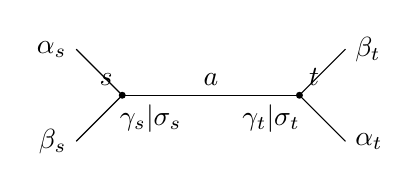
\begin{tikzpicture}[>=stealth,scale=.9]
\fill (0,0) circle (1.4pt) node[above left] {$s$};
\fill (2.5,0) circle (1.4pt) node[above right] {$t$};
\draw (0,0)--(2.5,0) node[midway,above] {$a$};
\draw (0,0)--(-.65,.65) node[left] {$\alpha_s$};
\draw (0,0)--(-.65,-.65) node[left] {$\beta_s$};
\draw (2.5,0)--(3.15,.65) node[right] {$\beta_t$};
\draw (2.5,0)--(3.15,-.65) node[right] {$\alpha_t$};
\node[below] at (.4,0) {$\unsure{\gamma_s|\sigma_s}$};
\node[below] at (2.1,0) {$\unsure{\gamma_t|\sigma_t}$};
\end{tikzpicture}}


\[
\underbrace{\alpha_s+\beta_s}_{\unsure{\gamma'_s|\sigma'_s}}
=
\underbrace{\alpha_t+\beta_t}_{\unsure{\gamma'_t|\sigma'_t}}
\]
et \unsure{=} la \uline{donnée} d'un \deleted{\unsure{isom}} \inserted{anti-}isom des torseurs sous $\unsure{\mathbb Z|\mathbf Z}/\unsure{\gamma|\sigma}$ $(\unsure{\gamma|\sigma}=\unsure{\gamma'_s|\sigma'_s}=\unsure{\gamma'_t|\sigma'_t})$
\[
\substack{\text{somme circulaire}\\\text{de }[1,\alpha_s]\text{ et }[1,\beta_s]}
\ \unsure{\simeq}\
\substack{\text{somme circulaire de}\\{}[1,\alpha_t]\text{ et }[1,\beta_t]}.
\]}

\deleted{\figure{\begin{tikzpicture}[scale=.6]
\coordinate (p) at (1,2); \coordinate (q) at (3,1.3);
\coordinate (r) at (2.7,.1); \coordinate (s) at (1,-.4);
\coordinate (t) at (0,.6);
\draw (p)--(q)--(r)--(s)--(t)--cycle;
\draw (p)--(.8,3.2) (q)--(4.5,1.9) (r)--(3.4,-.7) (s)--(1.1,-1.7) (t)--(-1,-.5);
\fill (r) circle (2pt);
\end{tikzpicture}}

}

\figure{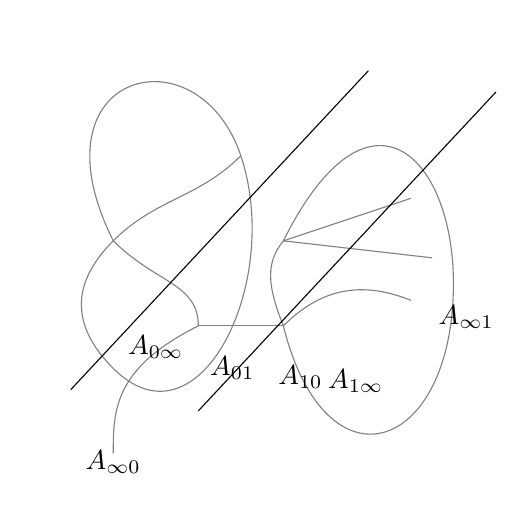
\begin{tikzpicture}[scale=.54,gray]
\draw (-3,1) .. controls (-5,5) and (-1,6) .. (0,3) .. controls (1,0) and (-1,-4) .. (-3,-2) .. controls (-4,-1) and (-4,0) .. (-3,1);
\draw (-3,1) .. controls (-2,2) and (-1,2) .. (0,3);
\draw (-3,1) .. controls (-2,0) and (-1,0) .. (-1,-1);
\draw (-1,-1) .. controls (-3,-2) and (-3,-3) .. (-3,-4);
\draw (1,1) .. controls (3,5) and (5,3) .. (5,0) .. controls (5,-4) and (2,-5) .. (1,-1) .. controls (.6,0) and (.6,.5) .. (1,1);
\draw (1,1)--(4,2);
\draw (1,1)--(4.5,.6);
\draw (1,-1) .. controls (2,0) and (3,0) .. (4,-.4);
\draw (-1,-1)--(1,-1);
\node[black] at (-3,-4.2) {$A_{\infty0}$};
\node[black] at (-2,-1.5) {$A_{0\infty}$};
\node[black] at (-.2,-2) {$A_{01}$};
\node[black] at (1.4,-2.2) {$A_{10}$};
\node[black] at (2.7,-2.3) {$A_{1\infty}$};
\node[black] at (5.3,-.8) {$A_{\infty1}$};
\draw[black] (-4,-2.5)--(3,5);
\draw[black] (-1,-3)--(6,4.5);
\end{tikzpicture}}
% crop-candidate: scan 67



\figure{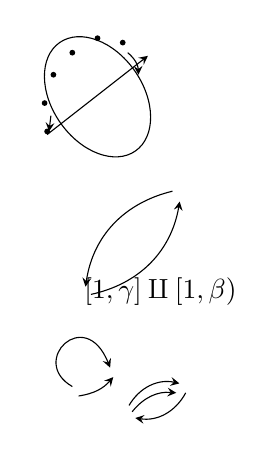
\begin{tikzpicture}[>=stealth,scale=.8]
\draw[rotate=35] (0,0) ellipse (.72 and 1.05);
\draw[->] (-.8,-.6)--(.8,.65);
\foreach \x/\y in {-.8/-.55,-.84/-.1,-.7/.35,-.4/.7,0/.93,.4/.86}
 \fill (\x,\y) circle (1.3pt);
\draw[->] (.48,.7) to[bend left=24] (.65,.35);
\draw[->] (-.74,-.3)--(-.77,-.55);
\begin{scope}[shift={(.6,-2.4)},rotate=35]
\draw[->] (-1,-.2) to[bend right=34] (1,.2);
\draw[->] (1,.4) to[bend right=34] (-1,-.05);
\end{scope}
\node at (1,-3.1) {$\unsure{[1,\gamma]\amalg[1,\beta)}$};
\draw[->] (-.4,-4.6) .. controls (-1.1,-4.2) and (-.2,-3.3) .. (.2,-4.3);
\draw[->] (-.3,-4.75) to[bend right=20] (.25,-4.45);
\draw[->] (.5,-4.9) to[bend left=36] (1.3,-4.55);
\draw[->] (1.4,-4.7) to[bend left=35] (.6,-5.1);
\draw[->] (.55,-5) to[bend left=28] (1.25,-4.7);
\end{tikzpicture}}



\[
\begin{array}{rcl}
\beta+\unsure{\gamma|\sigma}&=&\alpha'\\
\unsure{\gamma|\sigma}+\alpha&=&\beta'\\
\alpha+\beta&=&\unsure{\gamma'|\sigma'}
\end{array}
\qquad
\begin{array}{rcl}
\alpha&=&\dfrac{\beta'+\unsure{\gamma'|\sigma'}-\alpha'}2
=\dfrac{\alpha'+\beta'+\unsure{\gamma'|\sigma'}}2-\alpha'\\[3pt]
\beta&=&\dfrac{\unsure{\gamma'|\sigma'}+\alpha'-\beta'}{\unsure{2}}\\[3pt]
\unsure{\gamma|\sigma}&=&\dfrac{\alpha'+\beta'-\unsure{\gamma'|\sigma'}}2
\end{array}
\]
\[
\unsure{2(\alpha+\beta+\gamma)=\alpha'+\beta'+\gamma'},
\qquad
\unsure{2\alpha+\beta+\gamma=\beta'+\gamma'},
\qquad
\unsure{\beta+\gamma=\alpha'}.
\]
\[
\deleted{\unsure{\alpha}},\quad
\unsure{(\alpha'+\beta'-\gamma')-(\beta+\gamma)},\quad
\unsure{\alpha'},\quad
\unsure{\dfrac{\alpha'+\beta'+\gamma'}2}.
\]

\figure{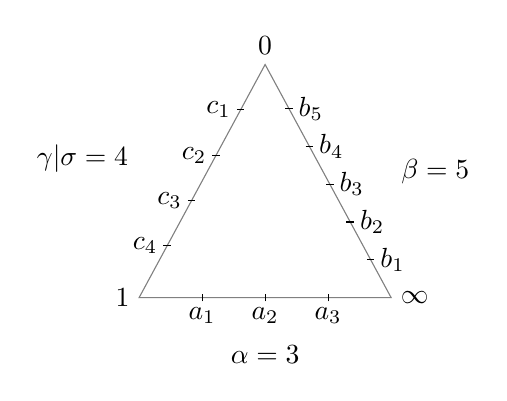
\begin{tikzpicture}[scale=.8]
\draw[gray] (0,0)--(2,3.7)--(4,0)--cycle;
\node[above] at (2,3.7) {$0$}; \node[left] at (0,0) {$1$}; \node[right] at (4,0) {$\infty$};
\foreach \i in {1,2,3} {
 \pgfmathsetmacro{\x}{\i}
 \draw (\x,-.06)--(\x,.06); \node[below] at (\x,0) {$a_\i$};
}
\foreach \i in {1,2,3,4} {
 \pgfmathsetmacro{\y}{3.7-.72*\i}
 \pgfmathsetmacro{\x}{2*\y/3.7}
 \draw (\x-.06,\y)--(\x+.06,\y); \node[left] at (\x,\y) {$c_\i$};
}
\foreach \i in {1,2,3,4,5} {
 \pgfmathsetmacro{\y}{.6*\i}
 \pgfmathsetmacro{\x}{4-2*\y/3.7}
 \draw (\x-.06,\y)--(\x+.06,\y); \node[right] at (\x,\y) {$b_\i$};
}
\node at (-.9,2.2) {$\unsure{\gamma|\sigma}=4$};
\node at (4.7,2) {$\beta=5$};
\node at (2,-.9) {$\alpha=3$};
\end{tikzpicture}}



\figure{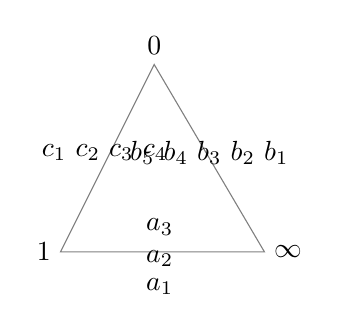
\begin{tikzpicture}[scale=.7]
\draw[gray] (0,0)--(1.7,3.4)--(3.7,0)--cycle;
\node[above] at (1.7,3.4) {$0$}; \node[left] at (0,0) {$1$}; \node[right] at (3.7,0) {$\infty$};
\node at (.8,1.8) {$c_1\ c_2\ c_3\ c_4$};
\node at (2.7,1.8) {$b_5\ b_4\ b_3\ b_2\ b_1$};
\node at (1.8,.45) {$a_3$}; \node at (1.8,-.12) {$a_2$}; \node at (1.8,-.63) {$a_1$};
\end{tikzpicture}}



\figure{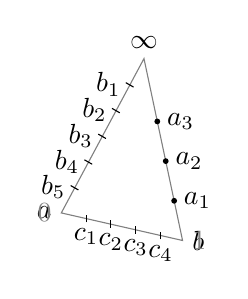
\begin{tikzpicture}[scale=.7]
\draw[gray] (0,0)--(1.5,2.8)--(2.2,-.5)--cycle;
\node[above] at (1.5,2.8) {$\infty$}; \node[left] at (0,0) {$\unsure{a}$}; \node[right] at (2.2,-.5) {$\unsure{b}$};
\node[gray,left] at (0,0) {$0$}; \node[gray,right] at (2.2,-.5) {$1$};
\foreach \i in {1,2,3,4,5} {
 \pgfmathsetmacro{\x}{1.5-.25*\i}
 \pgfmathsetmacro{\y}{2.8-.4667*\i}
 \draw (\x-.08,\y+.03)--(\x+.06,\y-.05); \node[left] at (\x,\y) {$\unsure{b_\i}$};
}
\foreach \i in {1,2,3} {
 \pgfmathsetmacro{\y}{-.5+.72*\i}
 \pgfmathsetmacro{\x}{2.2-.7*(\y+.5)/3.3}
 \fill (\x,\y) circle (1.5pt); \node[right] at (\x,\y) {$\unsure{a_\i}$};
}
\foreach \i in {1,2,3,4} {
 \pgfmathsetmacro{\x}{.45*\i}
 \pgfmathsetmacro{\y}{-.5*\x/2.2}
 \draw (\x,\y-.07)--(\x,\y+.07); \node[below] at (\x,\y) {$\unsure{c_\i}$};
}
\end{tikzpicture}}



\uline{NB} $\alpha',\beta',\unsure{\gamma'|\sigma'}$ \unsure{OK} ssi $\alpha'+\beta'+\unsure{\gamma'|\sigma'}$ pair

\figure{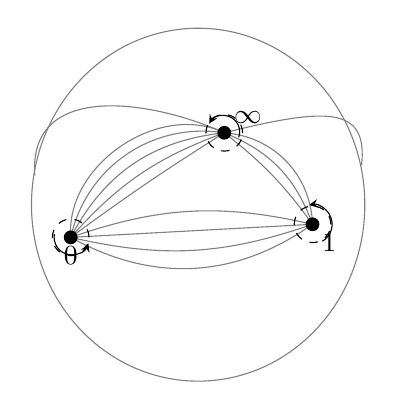
\begin{tikzpicture}[scale=.83,>=stealth]
\draw[gray] (0,0) ellipse (2.55 and 2.7);
\coordinate (z) at (-1.95,-.5); \coordinate (o) at (1.75,-.3); \coordinate (i) at (.4,1.1);
\foreach \b in {16,0,-16,-32} \draw[gray] (z) to[bend left=\b] (o);
\foreach \b in {2,14,28,43,60} \draw[gray] (z) to[bend left=\b] (i);
\foreach \b in {8,24,42} \draw[gray] (i) to[bend left=\b] (o);
\draw[gray] (-2.5,.45) .. controls (-2.6,1.9) and (-.7,1.6) .. (i)
 .. controls (2,1.5) and (2.6,1.5) .. (2.5,.6);
\foreach \p in {z,o,i} {\fill (\p) circle (3pt); \draw[dashed] (\p) circle (.28);}
\node[below] at (z) {$0$}; \node[below right] at (o) {$1$}; \node[above right] at (i) {$\infty$};
\draw[->] (-2.2,-.45) arc (170:340:.27);
\draw[->] (1.9,-.56) arc (-60:100:.3);
\draw[->] (.62,1.03) arc (-20:150:.25);
\end{tikzpicture}}



\[
\begin{array}{l|l}
\text{trois sommets}&\text{sommets d'ordre }\alpha',\beta',\unsure{\gamma'|\sigma'}\\
\alpha+\beta+\unsure{\gamma|\sigma}\ \text{arêtes}&
\end{array}
\]
\deleted{$\unsure{\alpha+\beta+\gamma}$}
\[
\left\{\begin{array}{ll}
(\alpha-1)+(\beta-1)+(\unsure{\gamma|\sigma}-1)&
\overbrace{\text{faces-bigones}}^{=\alpha+\beta+\unsure{\gamma|\sigma}-\unsure{2}}\\
2&\text{faces-triangles}
\end{array}\right.
\quad\bigg|\quad \alpha+\beta+\unsure{\gamma|\sigma}-1\ \text{faces}
\]
\mspage{66}
